\newpage
\section{Design approach}
\label{s:design}

As shown, no existing solution fully covers the described use cases, and this mandates further research. This section defines requirements for a system that would be more suitable for ESTCube-2 than any existing alternatives. Possible design for meeting those requirements is also proposed.

\subsection{Requirements}

Software updating system that would be more suitable for ESTCube-2 than any existing alternatives, must:

\begin{enumerate}
	\item allow addition of program code without the need to re-transmit significant portions of already existing code, so that it could be used for small one-time subroutines as well.
	\item allow changing a subset of existing code without the need to re-transmit significant portions of unchanged code, so that upload bandwidth and update application time would be minimized.
	\item not require on-board modifications of uploaded code. This makes it possible to store code directly in internal flash in the case that external memory modules are unavailable.
	\item make it possible to rearrange functions on board. This enables defragmenting the internal flash.
	\item not depend on \gls{os} features that are unavailable in a standard distribution of Free\-RTOS, since this is the \gls{os} planned for ESTCube-2 \gls{obc}.
	\item not significantly reduce code performance compared to a system that uses full image replacement.
	\item support full inter-component communication. This enables any unforeseen updates as well, which a predefined \gls{api} could limit.
\end{enumerate}

\subsection{Proposed solution}

% divided into firmware and functions
The proposed solution divides on-board software into two parts: firmware (startup script, \gls{hal}, \gls{os}, and critical device drivers) and application software (everything else) (Figure~\ref{fig:swOrg}). Firmware would be updatable by means of full image replacement, similar to how updates worked on ESTCube-1, including the use of multiple versions. This is proposed since firmware is expected to be updated rarely, if ever, and is too critical to use experimental updating methods with it.

\begin{figure}[ht]
	\centering
	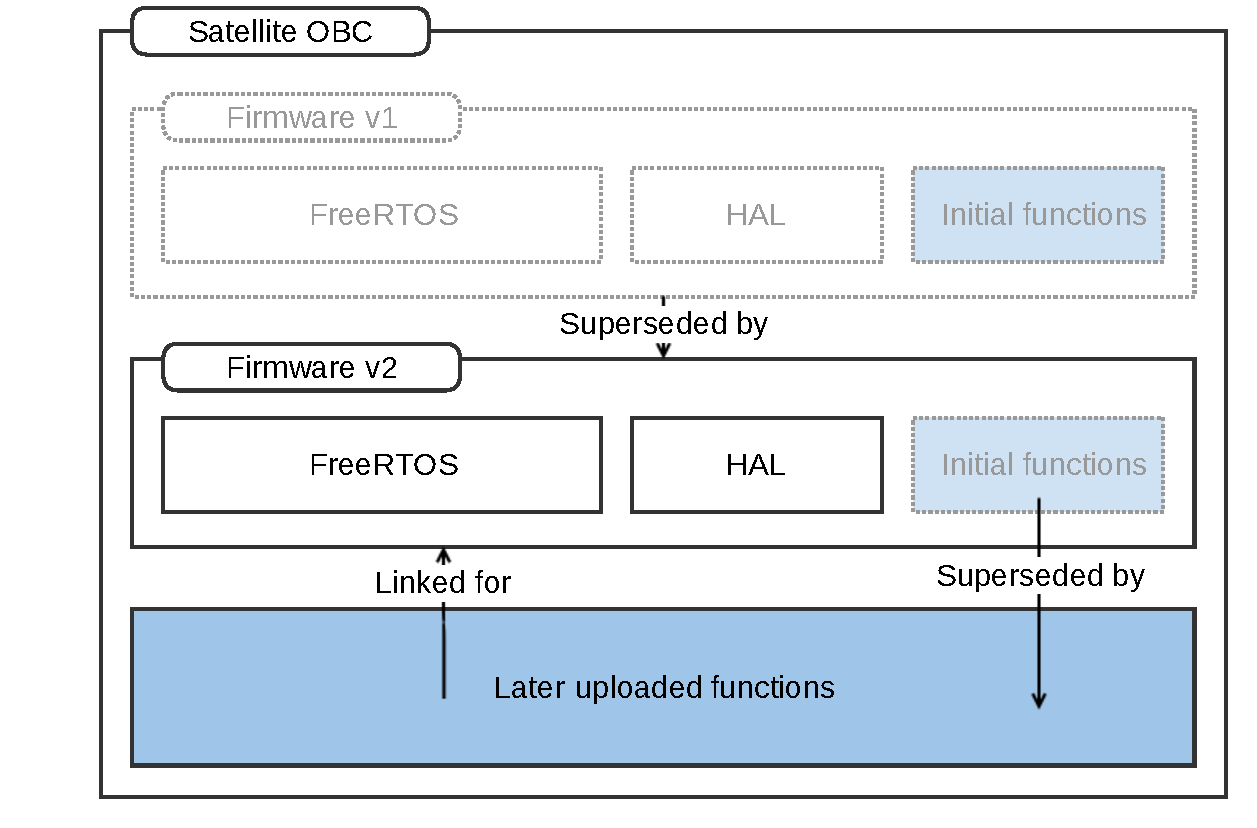
\includegraphics[width=0.9\textwidth]{figures/On-board_software_organization.pdf}
	\caption{Proposed on-board software organization. Blue denotes application software.}
	\label{fig:swOrg}
\end{figure}

% divided by function
Application software, on the other hand, would be divided into parts, each containing a single function. Each application function would be combined with a short header (Table~\ref{tab:header}) to form a package. Each function could then be independently updated, added or removed.

\begin{table}[ht]
	\centering
	\caption{Application function's header.}
	\begin{tabular}{r|l|l}
		\bf{Length (bytes)} & \bf{Field} & \bf{Format} \\
		\hline
		4 & \Gls{crc} & CRC-32 \\
		\hline
		1 & Type &
		\begin{tabular}{r|l}
			\texttt{0xff} & nothing \\
			\texttt{0xaa} & function \\
			\texttt{0x55} & global \\
			\texttt{0x00} & disabled \\
		\end{tabular} \\
		\hline
		2 & Function ID & uint16 \\
		\hline
		1 & Version no & uint8 \\
		\hline
		2 & Length of body & uint16 \\
		\hline
		2 & \Gls{sram} offset (global variables only) & uint16 \\
	\end{tabular}
	\label{tab:header}
\end{table}

% padding
The headers (Table~\ref{tab:header}) will have \texttt{nop}-instructions appended to them to pad them to 12 bytes in length. Some instructions will generate a fault or will execute slower if addresses are not word-aligned \cite[Section~3.3.5]{STMicroelectronics2017}, therefore a multiple of 4 bytes was chosen for the header length.

% snapshots
Function version dependencies would be managed by a system of snapshots similar to git \cite[Chapter~1.3]{Chacon2018}: after new functionality has been developed and tested, current version of all functions is recorded. \Gls{mcs} will then determine, which of them differ when compared to satellite's internal storage, and upload those.

\subsubsection{On-board storage of application software}

Main focus is on storing application functions in internal flash, since it is the most restrictive storage. Additionally, in safe mode, this is the sole non-volatile storage available (Section~\ref{s:hardware}). Storage of some functions in other memories, as well as moving functions between different memories and addresses, would also be possible.

While flash memory does not support deleting or changing any data short of an entire sector, new data can be appended. Functions would therefore be written to flash sequentially as they arrive. Additionally, flash allows the addition of zeros into data. This way functions could be marked as disabled by replacing some predefined area of function header with zeros ('Type' in Table~\ref{tab:header}), without the need to delete the sector. In order to change a function, a new version would simply be appended to the storage. If several versions of a function are found in memory, the last one will be considered correct.

\subsubsection{Linking}

Compiled code contains many symbol references: function calls, global variables, etc. For software to run, all of them must be replaced with absolute memory addresses. In order to satisfy all requirements (especially about no modifications to uploaded code), a combination of static pre-linking and custom dynamic linker would be used.

Firmware would be compiled and linked to a fixed memory address first - meaning that absolute memory addresses of all functions and global variables in the firmware would be fixed. This way calls to all firmware functions from other firmware functions, as well as from any later added application functions, can be simply linked on the ground (Figure~\ref{fig:swLink}).

\begin{figure}[ht]
	\centering
	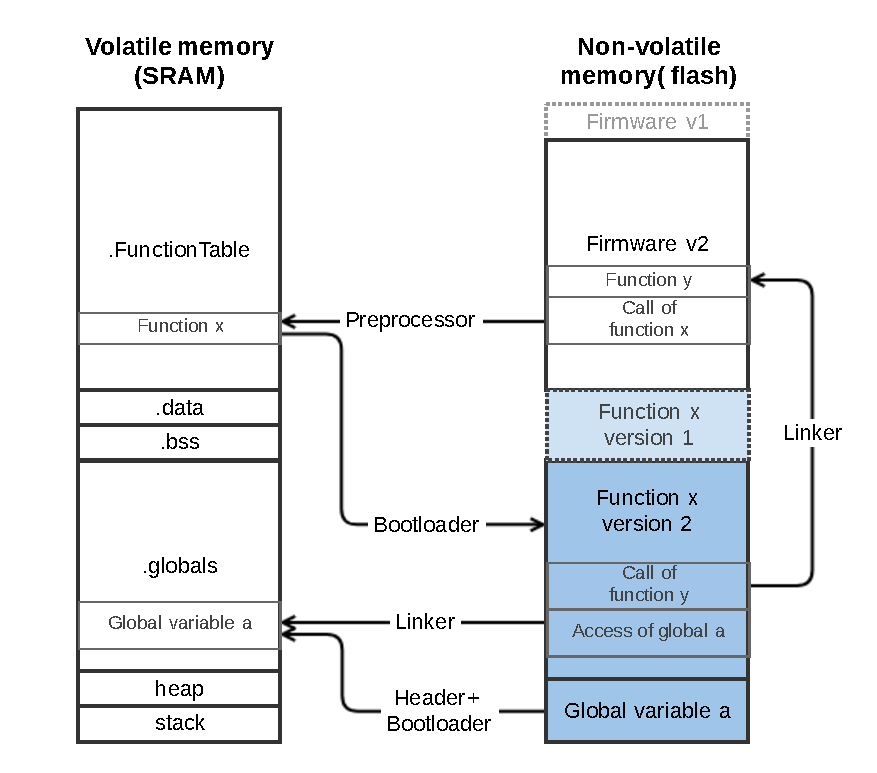
\includegraphics[width=0.96\textwidth]{figures/Software_linking.pdf}
	\caption{References in on-board software. Blue denotes application software.}
	\label{fig:swLink}
\end{figure}

Calling application functions is more tricky, as they can move around in memory. They would be callable by using a system-global offset table (Figure~\ref{fig:swLink}). This table would contain the current memory address for each function. It will be stored in volatile internal \gls{sram} and re-created every time the system boots (by walking over all stored functions and storing the address where each function appears last). The table itself would be located on fixed memory location and contain functions sorted by id. It can be also changed during the run-time, when new functions are added. Changing it during the run-time when a function is changed requires additional checks to guarantee that previous memory address does not remain in use (as some function pointer somewhere) and is therefore out of the scope of this work, but is a potential future improvement.

Additionally, firmware can't call functions, whose signatures are not known at the time of firmware compilation, since compiler must generate code for passing arguments. For that reason, some functions are bundled with the firmware (Figure~\ref{fig:swOrg}). Examples would include functions dealing with the \gls{icp} and software updating itself. They can be updated, but their signatures must remain unchanged.

The table of function offsets would be periodically checked for errors. Functions' checksums could also be checked during the generation of this table. During reboot, flash memory can also be defragmented.

\subsubsection{Compiling application functions}

Compilers support generating indirect function calls out of the box for \gls{pic}. However, the commonly-used \gls{svr4} scheme expects the \gls{got} to be at a fixed offset from the code \cite[Chapter~8]{Levine1999}. This has the effect that each independent portion of code needs its own copy of the \gls{got}, but having one for each function would cause unacceptable size overhead. To avoid having to modify the compiler itself, a way to rewrite all function calls using the preprocessor will be used.

For each function that would otherwise result in an unresolved external symbol, a preprocessor macro (Figure~\ref{fig:macro}) will be generated. It contains instructions to read function's address from the function table, cast it to the function's type, cast all arguments to required types, and call the function. Since the macro call syntax will be identical to that of a function call, application code can be agnostic to the updating platform.

\begin{figure} [htb]
\begin{lstlisting}[language=C]
typedef void (*f0_t)();
#define f0() (*((f0_t)(*((uint32_t *) (0x20000000)))))()
\end{lstlisting}
\caption{Call interception macro for the hypothetical function \texttt{f0()} with id 0, where the function table is located at a fixed address \texttt{0x20000000}.}
\label{fig:macro}
\end{figure}

For calling important functions, the checksum of the function can be checked immediately before jumping by incorporating modified interception macro. Normally this is not done.

\subsubsection{Global variables}

In order to simplify the design, global variables would be treated very similarly to functions. First, they would be compiled, since then the the compiler would calculate their lengths. Compilation should include the flag \texttt{-fdata-sections}, this way they can be extracted to separate packages, prepended with headers, and uploaded to the satellite.

Memory space after \texttt{.data} and before heap would be reserved for updatable global variables  (Figure~\ref{fig:swLink}). Linker would select an address for each variable in that area, and then all functions using the variable could be statically pre-linked on the ground. Headers for global variables would contain the appropriate type, and additionally the memory address allocated for this variable (Table~\ref{tab:header}). During boot, when function addresses are being added to the offset table, global variables would be copied to their respective addresses (Appendix~\ref{apx:gentable}). As with a function, the latest occurrence of a global variable overrides any previous ones.
